\begin{figure}
  \centering
  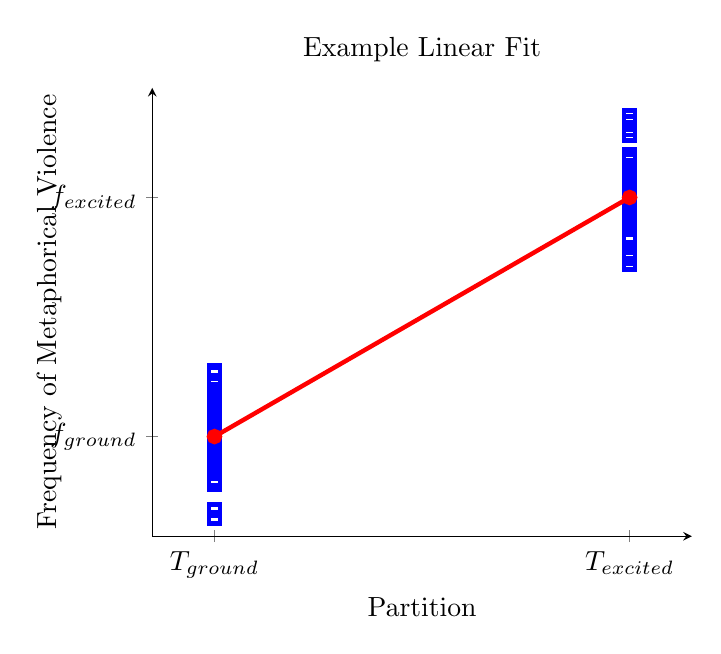
\begin{tikzpicture}
    \begin{axis}[
      ,title=Example Linear Fit
      ,axis x line = bottom, axis y line = left
      ,xlabel=Partition
      ,y label style={at={(axis description cs:-0.15,.5)}}
      ,ylabel=Frequency of Metaphorical Violence
      ,xmin=-.15, xmax=1.15
      ,ymin=0, ymax=2.25
      ,xtick={0, 1}
      ,xticklabels={$T_{ground}$, $T_{excited}$}
      ,ytick={0.5, 1.7} 
      ,yticklabels={$f_{ground}$, $f_{excited}$}
      ,every axis plot/.append style={ultra thick}
      ,clip marker paths=true
      ,anchor=origin
      ]
      \addplot+[only marks, mark=square, blue] coordinates {
        (0, 0.28176763326) (0, 0.350579774235) (0, 0.494762486627) (0, 0.698017229947) (0, 0.0914119670018) (0, 0.562791554989) (0, 0.414408243237) (0, 0.448752389982) (0, 0.534869456009) (0, 0.565298122439) (0, 0.713342069417) (0, 0.570802600869) (0, 0.600080420076) (0, 0.339212985545) (0, 0.536222381064) (0, 0.325157942968) (0, 0.482143784654) (0, 0.651252469343) (0, 0.262656739438) (0, 0.734264833239) (0, 0.527160094444) (0, 0.670540313522) (0, 0.782590258513) (0, 0.544998389383) (0, 0.406587061347) (0, 0.13090649078) (0, 0.325595587657) (0, 0.467227203324) (0, 0.26067945992) (0, 0.42655727858) (0, 0.280874951953) (0, 0.627523159582) (0, 0.52163666621) (0, 0.689592043265) (0, 0.582769397727) (0, 0.707024689504) (0, 0.598615409781) (0, 0.347973302243) (0, 0.360956698235) (0, 0.699323678165) (0, 0.819275219019) (0, 0.832535941995) (0, 0.572485985687) (0, 0.727924580262) (0, 0.41724329832) };
      \addplot+[only marks, mark=square, blue] coordinates {
        (1.0, 1.91247092918) (1.0, 1.5394596921) (1.0, 2.10773281394) (1.0, 1.89887130293) (1.0, 1.61425294087) (1.0, 1.71383269787) (1.0, 1.8310274463) (1.0, 1.73530670109) (1.0, 1.40727197112) (1.0, 1.82023604091) (1.0, 1.63965557868) (1.0, 1.73899638436) (1.0, 1.36919392698) (1.0, 1.58641297881) (1.0, 1.83803888564) (1.0, 1.71802566345) (1.0, 1.68759269019) (1.0, 2.01343061625) (1.0, 1.60507200871) (1.0, 1.79480251021) (1.0, 1.36483678083) (1.0, 1.85793134182) (1.0, 1.56941110605) (1.0, 1.4855004683) (1.0, 1.76177910132) (1.0, 1.58485972151) (1.0, 1.5846086847) (1.0, 1.48354037111) (1.0, 2.04198439011) (1.0, 1.6987951821) (1.0, 1.44801569567) (1.0, 2.07846405613) (1.0, 1.80107745091) (1.0, 1.3956308386) (1.0, 1.62193882796) (1.0, 1.55818973594) (1.0, 1.8896926668) (1.0, 1.71657899717) (1.0, 1.58108619149) (1.0, 1.59786892921) (1.0, 1.66832037628) (1.0, 1.83181642753) (1.0, 1.79348201084) (1.0, 1.88734472296) (1.0, 1.62566264372)
      };
      \addplot+[red] coordinates { (0, .5) (1.0, 1.7) };
    \end{axis}
  \end{tikzpicture}
  \caption{Each model corresponding to a pair of partition times, $(\tau_1^*, \tau_2^*)$,
  is a linear fit. The linear model that minimizes the AIC is considered the
  most likely to minimize information loss. We fit about 1,000 linear models
  to the coded data just like this one. Once the optimal pair $(\tau_1^*, \tau_2^*)$
  has been identified, we obtain $f_{ground}$ and $f_{excited}$ as identified in the linear fit.
  }
\label{fig:linear-model-illustration}
\end{figure}
